%; whizzy document
% latex beamer presentation.
% platex, latex-beamer でコンパイルすることを想定。 

%     Tokyo Debian Meeting resources
%     Copyright (C) 2007 Junichi Uekawa

%     This program is free software; you can redistribute it and/or modify
%     it under the terms of the GNU General Public License as published by
%     the Free Software Foundation; either version 2 of the License, or
%     (at your option) any later version.

%     This program is distributed in the hope that it will be useful,
%     but WITHOUT ANY WARRANTY; without even the implied warranty of
%     MERCHANTABILITY or FITNESS FOR A PARTICULAR PURPOSE.  See the
%     GNU General Public License for more details.

%     You should have received a copy of the GNU General Public License
%     along with this program; if not, write to the Free Software
%     Foundation, Inc., 51 Franklin St, Fifth Floor, Boston, MA  02110-1301 USA

% 実行順番
% sudo  ~/bin/usb-macbook-ir.c &
% real presentation (shell-command (concat "DISPLAY=:0.1 xpdf -fullscreen " (replace-regexp-in-string "tex$" "pdf"(buffer-file-name)) "&"))
% DISPLAY=:0.1 xpdf -fullscreen 

\documentclass[cjk,dvipdfmx]{beamer}
\usetheme{Tokyo}

%  preview (shell-command (concat "xpdf " (replace-regexp-in-string "tex$" "pdf"(buffer-file-name)) "&"))
%  presentation (shell-command (concat "xpdf -fullscreen " (replace-regexp-in-string "tex$" "pdf"(buffer-file-name)) "&"))

%http://www.naney.org/diki/dk/hyperref.html
%日本語EUC系環境の時
\AtBeginDvi{\special{pdf:tounicode EUC-UCS2}}
%シフトJIS系環境の時
%\AtBeginDvi{\special{pdf:tounicode 90ms-RKSJ-UCS2}}

\title{東京エリア Debian 勉強会}
\subtitle{資料}
\author{上川 純一 dancer@debian.org\\IRC nick: dancerj}
\date{2007年3月17日}
\logo{
\includegraphics[width=8cm]{image200607/openlogo-light.eps}}

% 三択問題用
\newcounter{santakucounter}
\newcommand{\santaku}[5]{%
\addtocounter{santakucounter}{1}
\frame{\frametitle{問題\arabic{santakucounter}. #1}
%問題\arabic{santakucounter}. #1
\begin{minipage}[t]{0.8\hsize}
 \begin{itemize}
 \item 
\includegraphics[width=0.2\hsize]{image200703/janken-A.png} A #2\\
 \item 
\includegraphics[width=0.2\hsize]{image200703/janken-B.png} B #3\\
 \item 
\includegraphics[width=0.2\hsize]{image200703/janken-C.png} C #4\\
 \end{itemize}
\end{minipage}
}
\frame{\frametitle{問題\arabic{santakucounter}. #1}
%問題\arabic{santakucounter}. #1
\begin{minipage}[t]{0.8\hsize}
\begin{itemize}
 \item 
\includegraphics[width=0.2\hsize]{image200703/janken-A.png} A #2\\
 \item 
\includegraphics[width=0.2\hsize]{image200703/janken-B.png} B #3\\
 \item 
\includegraphics[width=0.2\hsize]{image200703/janken-C.png} C #4\\
\end{itemize}
\end{minipage}
\begin{minipage}[t]{0.15\hsize}
答えは:

\vspace{1cm}

  {\huge \hspace{1cm}#5}
  \hspace{-6cm}\includegraphics[width=4cm]{image200703/janken-#5.png}
 \end{minipage}}
}

\begin{document}
\frame{\titlepage{}}

\section{Intro}

\begin{frame}
 \frametitle{本日のagenda}
\begin{minipage}[t]{0.4\hsize}
  \begin{itemize}
   \item 仮想化友の会、Debian 勉強会の紹介
   \item 事前課題紹介
   \item 仮想化常識Quiz
 \end{itemize}
\end{minipage} 
\begin{minipage}[t]{0.4\hsize}
 \begin{itemize}
   \item Windowsから見える仮想化世界
   \item Debianの仮想化技術紹介
   \item 最後に
 \end{itemize}
\end{minipage}
\end{frame}

\section{Debian 勉強会の紹介}
\begin{frame}{}

{Debian勉強会の紹介}
 
\end{frame}

\subsection{東京エリア Debian 勉強会とは}

\begin{frame}{東京エリア Debian 勉強会とは?}
\begin{itemize}
  \item<1-> Debian Developer である 上川 純一 が発起人
  \item<2-> 2005年1月から開始
  \item<3-> 月に1回コンスタントに勉強会を行っている
  \item<4-> 場所は荻窪にある公民館(あんさんぶる荻窪)
\end{itemize}
\end{frame}

\subsection{勉強会 の目的}

\begin{frame}{勉強会 の目的}
\begin{itemize}
  \item<1-> 現状は ML と IRC と WEB だけが情報源、情報交換に限りがある
  \item<2-> 実際にface to face で話し合える場所がない
  \item<3-> 情報が断片的で、まとまったドキュメントがない
\end{itemize}
\end{frame}

\begin{frame}
 \frametitle{勉強会 の目的}
\begin{itemize}
  \item<1-> 定期的に集まれる場所を作ろう
  \item<2-> 勉強会を行うときは必ず資料を作成する
  \item<3-> もちろん、資料は DFSG Free、Webサイトで公開 
\footnote{http://tokyodebian.alioth.debian.org}
  \item<4-> 最終的にはみんなガリガリパッケージを作れるように
\end{itemize}
\end{frame}

\subsection{勉強会 の内容}
\begin{frame}
 \frametitle{勉強会 の内容}
\begin{itemize}
  \item<1-> Debian Weekly News Quiz
  \item<2-> 毎回 Debian に関する マニアックなお題
    \begin{itemize}
	\item Debian Policy について
	\item dpatch / quilt / dbs の使いかた
	\item Debconf 現地からの報告
	\item などなど
    \end{itemize}
  \item<3-> もちろん Debian に関するユーザー向けの話題もやってます
    \begin{itemize}
	\item Macbook on Debian
	\item Debian sid へいざない
	\item BTS のしかた
	\item などなど
    \end{itemize}
  \item<4-> GPG キーサインパーティ
  \item<5-> 宴会という名の交流会
\end{itemize}
\end{frame}

\subsection{勉強会を行ってからの結果}
\begin{frame}
 \frametitle{勉強会 を行ってからの結果}
\begin{itemize}
  \item<1-> Debian Package メンテナーが増えた
    \begin{itemize}
	\item 小林さん
	\item やまねさん
	\item 三塚さん
	\item 岩松
    \end{itemize}	
  \item<2-> Debian Developer 予備軍が増えた
  \item<3-> Debian に関する資料が増えた
  \item<4-> Debian での日本語の環境がよくなりつつある
  \item<5-> Debian JP Project の正式勉強会になった
  \item<6-> 出張 Debian 勉強会を行うようになった
    \begin{itemize}
	\item 北海道
	\item 大阪
    \end{itemize}	
\end{itemize}
\end{frame}

\begin{frame}
 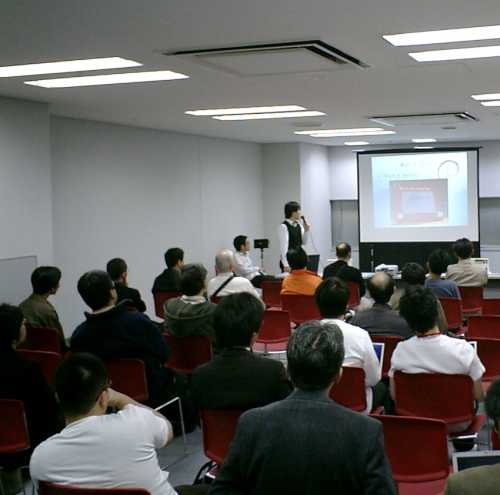
\includegraphics[width=0.8\hsize]{image200611/meeting.jpg}
\end{frame}

\begin{frame}{メンバーのメンテナンスしているパッケージ例}
 \begin{itemize}
 \item 山根さん: eclipse-nls, jd, ttf-vlgothic
 \item 岩松さん: flash, tinywm, ttf-mona
 \item 小林さん: serf, skkdic, skksearch
 \item みつかさん: canna
 \item えとーさん: qwik
 \end{itemize}
\end{frame}

\subsection{今後の予定しているお題}
\begin{frame}
 \frametitle{今後の予定しているお題}
\begin{itemize}
  \item darcs, quilt, git を Debian パッケージに活用する
  \item Debian インストールから実戦投入まで
  \item Debconf 7 報告会
\end{itemize}
\end{frame}

\subsection{今後の開催予定}
\begin{frame}
 \frametitle{今後の開催予定}
\begin{itemize}
  \item 2007年 4月 21日\\
	18:00 から 荻窪にて開催予定
  \item 2007年 5月 19日\\
	場所未定。
\end{itemize}
\end{frame}

\begin{frame}
 \frametitle{Web サイト}
\begin{itemize}
  \item 東京エリア Debian 勉強会 Web サイト\\
	\url{http://tokyodebian.alioth.debian.org}
\end{itemize}
\end{frame}

\section{仮想化友の会の紹介}
\begin{frame}{}

{仮想化友の会の紹介}
 
\end{frame}

\section{事前課題の声}
\begin{frame}{事前課題の声}

「仮想化を実際にこういう利用方法で活用しています」
 
 事前課題内容紹介

\end{frame}



%%% 

\subsection{前田 耕平さん}

\begin{frame}{}
 都内在住前田さん(2X歳・独身(仮))の場合
\end{frame}

\begin{frame}
{Windowsでしか使えないハードウェア(プリンタ・スキャナ・コピー複合機)を使うため}

 北側の部屋(サーバルーム兼図書室)に置いているミニタワー型PCのVMware上のWindowsを使うのに、
 SSHでXをポートフォワーディングさせて、和室のノートPCで使ってます。(北側の部屋は寒いので。)
 ちょうど今は、VMware上のWindowsをリモートで表示させて、
 確定申告の用紙を印刷するのにフル活用中。(年末は年賀状)
 普通にリモートデスクトップを使えば?というツッコミはなしでおねがいしま
 す。
 結局、プリンター((Epson CC-700))がWindowsでしか使えないからなのですが…
\end{frame}

\begin{frame}
{某社の暗号化ツール対応のため}

 秘文で暗号化したファイルは Windows の exe 形式のため、Linux上では複号で
 きないため、
 VMWareかKVM上のWindowsに一度ファイルを持っていって復号した後、復号済みのファイルを
 Linuxに持っていく、という使いかたをしています

\end{frame}

\begin{frame}
{Let's note の無線LANドライバを抽出するため}

 今使っている、Let's note R3は購入直後にきれいさっぱりWindowsを消しており、
 ndiswrapperでWindowsのドライバを使用するのに、Windowsが必要だったので
 
\begin{enumerate}
 \item PanasonicのサイトからドライバをVMware上のWindowsにダウンロード
 \item 普通に展開しようとすると、ハードウェアのチェックが入るので、
       lhaplusで解凍、tarballに圧縮
 \item tarballをLinuxに持っていき、展開してndiswrapperで使用
\end{enumerate}

 ipw2200がダメだったので、ndiswrapperに逃げた結果なのですが・・・
\end{frame}


\begin{frame}{別のディストロを試すため。}
 自宅のPCや鯖にはネイティブにはDebianを入れており、別のディストロを試すために、
 毎回入れ直すのが面倒になったので

 (前はテスト専用機で1ヶ月に一度くらいの頻度でいろんなディストロを入れ直してましたが)
\end{frame}

\subsection{Yoshihiro Yoshida さん}

\begin{frame}{}
仮想化友の会会員 Yoshihiro Yoshida さんの場合の仮想化利用方法
\end{frame}

\begin{frame}
{システムバックアップ}

  通常のサーバの場合、OSを含めたシステムバックアップの取得には、
  CDブートやシングルユーザでのブートが必要となり、サーバの台数が多いと
  時間のかかる作業となってしまいますが、仮想化ソフトを使用していれば、
  イメージファイルのバックアップだけですむため、バックアップ作業の時間が
  大幅に短縮できます
\end{frame}

\begin{frame}
{サーバリプレース}

  古い資産を使い続けたいのに、古いOSに対応するハードウェアが見つからない
  というケースが最近みられるのですが、そういった場合には無理にハード
  ウェアを探すのではなく、スペックに余裕のあるマシンに仮想化環境を構築
  し、そこで古い資産を動作させることが可能です
\end{frame}

\begin{frame}
{vmotion livemigrationによるノンストップ切り替え}

  どんなクラスタソフトでも運用機と待機機が切り替わる際にはサーバの停止が
  必要となってしまいます。しかし、VMotionやLive Migrationといった機能を
  使用することにより、サーバをノンストップで切り替えることが可能となります
\end{frame}

\begin{frame}
{サーバの配布に使用}

  東京でサーバのセッティングを行い、全国の各支店に送付するようなケース
  がまれにあるのですが、そのような場合にも仮想化ソフトを使用すれば筐体を
  東京に集める必要はなく、イメージを送付するだけでサーバの配布が可能と
  なります
\end{frame}

\begin{frame}
{インストーラの試験に使用}

  通常インストーラの試験を実施するためには、インストール、
  アンインストールを繰り返し実施する必要がありますが、仮想化ソフトの
  スナップショット機能を使用すると簡単にインストール前の状態に戻すことが
  できるため、効率的に試験を実施することが可能になります
\end{frame}

\begin{frame}
{アプリの異常系試験}

  通常の環境では躊躇してしまうような大胆な異常系の試験もスナップショット
  で簡単に環境を戻せることを考えれば、気軽に実施することが可能になりす
\end{frame}

\subsection{芝@岡山さん}

\begin{frame}{}
岡山県在住 芝さんの場合
\end{frame}

\begin{frame}
{旧環境の保存}

 旧バージョンのブラウザやフォント環境でcssのテストや
 アプリケーションの動作チェック、
 Visual Studio 6.0環境の保存ができる
\end{frame}

\begin{frame}
{ネットワーク環境のテスト}

 1マシン上で複数OSのクライアントサーバ環境がテスト出来る、
 開発時は高負荷かけないのでノートPCでも十分なときが多い
\end{frame}

\begin{frame}
{一時利用サーバ}

 常時使うわけではないので専用機を準備するのは勿体ない
 PXEサーバ等に活用
\end{frame}

\begin{frame}
{1CDLinuxで遊ぶ}

 Windows上の仮想環境からknoppix立ち上げることが多いような感じです
 仮想環境ですと焼かなくて済むのとディスクアクセスが速いので遊びやすいです
 実用例ですとドイツのネットカフェでqemuからknoppix立ち上げて日本語打ってました。

もう少し軽快になるとUSBメモリでHDDイメージ持ち歩くのが普通になるかもしれません。
メール環境やブラウザのクッキー持ち歩くとか考えるよりシンプルですよね

\end{frame}


\begin{frame}{}
東京都在住 Debian 勉強会 岩松さん(2X歳 独身)の場合
\end{frame}

\begin{frame}
{Debian installer のテスト}
 qemu を使って、Debian-installer のテストをしています。
\end{frame}

\begin{frame}
{別アーキテクチャ上のテスト}
 qemu を 実機を持っていない アーキテクチャのテストに使っています。
 Debian のパッケージメンテナンスを行う時に非常にありがたい存在です。
\end{frame}

\begin{frame}
{CPUのシミュレーションとして}
 実機がない場合でも、Linux カーネルの開発が行えるように、qemu を使っています。
 基板の設計と Linux カーネルの開発が同時に進行できるので、便利です。
\end{frame}

\begin{frame}
{他ディストリビューションを使う}
 複数のディストリビューションを使う時に Xen を使っています。
 コンパイラをチェックするときに、ディストリビューション毎にPCがあっては
 管理が面倒くさいので、Xen 上で 複数のディストリビューションを動かし、
 テストに使っています。
\end{frame}



\begin{frame}{}
Debian 勉強会 上川の場合
\end{frame}

\begin{frame}{goodbye-microsoft.comを試す}
WindowsからDebianがインストールできるらしいんですけど、Debian 上で動いて
 いる kvm で動いている Windows で Debian をインストールしてみました。

動いた動いた
\end{frame}

\begin{frame}{linux-vserver を試す}
気軽に試すために、linux-vserver を kvm 上でインストールして試してみまし
 た

仮想OSとして動いている Debian でインストールするとすぐに試せます

\texttt{apt-get install linux-image-vserver-686 util-vserver}

\end{frame}


\begin{frame}{PaSoRiを使う}

PaSoRi を使うために利用

\end{frame}

%%%



\section{常識クイズ}

\begin{frame}{仮想化常識クイズ}
仮想化は最近流行しています。ただ、猫も杓子も仮想化といっている現状、本当
に常識をただしく理解してますか?
OSCの会場に到達できるみなさまであれば問題ないとは思いますが、念のため確
認テストをさせていただきます。
\end{frame}

\subsection{仮想化の常識}

\santaku
{仮想化でのparavirtualization とはなにか}
{仮想用にOSが変更されている}
{パラパラで仮装する}
{並列で仮想化する}
{A}

\santaku
{Intel の VTって何?}
{「バレーボール取ってきて」}
{真空管(vacuum tube)}
{Intel社が提唱するCPUの仮想化支援の仕組}
{C}

\subsection{仮想化の利点}

\santaku
{Windows を仮想化環境で実行することによる利点は何か}
{Windows VISTA ではライセンスを考えくてすむようになる}
{Windows がフリーソフトウェアになる}
{Windows が Linux 上で動く}
{C}
% Windows VISTA の例

\subsection{仮想化の分類}

\santaku
{別途カーネルが独立して必要では無い仮想化実装はどれか}
{user-mode-linux}
{xen}
{openvz}
{C}

\santaku
{kvm はなぜカーネルのメインラインにマージされたか?}
{作者がイケメンだった}
{政治力}
{影響範囲のコードが小さい}
{C}

\santaku
{kvm は paravirtualization をどういう方式で実現しているか}
{仮想環境で実行されるLinuxカーネルが paravirt\underline{ }ops 機構を利用
し、VMCALL 命令を発行することでホストOSに連絡する}
{根性・気合い}
{愛情}
{A}

\subsection{仮想化の仕組の常識}

\santaku
{x86 CPU において VMEXIT を発行する命令として、代表例である CPUID 命令の OPCODEは下記のうちどれ
か。}
{0x55}
{0x0f 0xa2}
{0x5d}
{B}
% 55, 5d はそれぞれ push/pop ebx

\santaku
{AMD-VとIntel-VT の一番大きな違いは次のどれか}
{会社が違う}
{命令が違う}
{思い入れが違う}
{A}

\santaku
{Xen の Domain-U の U は何か}
{Unprivileged}
{User}
{Unix}
{A}

\santaku
{Xen という名前は何から由来したか}
{Xeno}
{作者の娘の名前}
{禅寺}
{A}

\santaku
{KVMはなんの略か}
{Keyboard Video Mouse}
{Kernel-based Virtual Machine}
{「これ持ってる?」「こんなビデオ持ってるぜ」}
{B}

\santaku
{i386 の場合の Domain-U の ring level は何?}
{1}
{2}
{3}
{A}

\subsection{Debian での常識}

\santaku
{Debian Project で推奨する仮想化の技術は?}
{xen}
{kvm}
{DFSGに合致するものならなんでもよい}
{C}


\section{Windows から見える仮想化世界}
\begin{frame}{Windows から見える仮想化世界}
 山根さん
\end{frame}

\section{Debian の仮想化技術紹介}
\begin{frame}{KVM}
 前田さん
\end{frame}

\begin{frame}{濃い話1}
 平さん:私はこれで○○を辞めました。
\end{frame}

\begin{frame}{KVM活用例}
 上川
\end{frame}

\begin{frame}[containsverbatim]{goodbye-microsoft.com を試す}
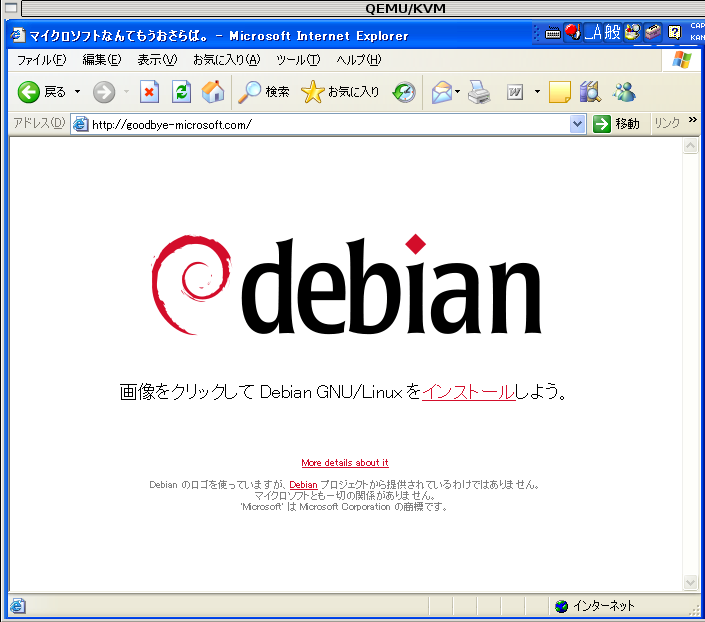
\includegraphics[width=10cm]{image200703/goodbyemicrosoftcom1.png}
\end{frame}
\begin{frame}[containsverbatim]{goodbye-microsoft.com を試す}
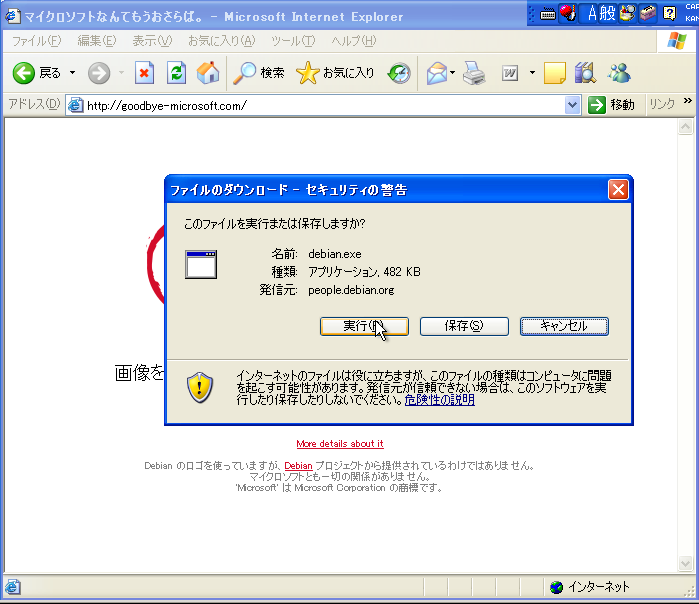
\includegraphics[width=10cm]{image200703/goodbyemicrosoftcom2.png}\\
\end{frame}
\begin{frame}[containsverbatim]{goodbye-microsoft.com を試す}
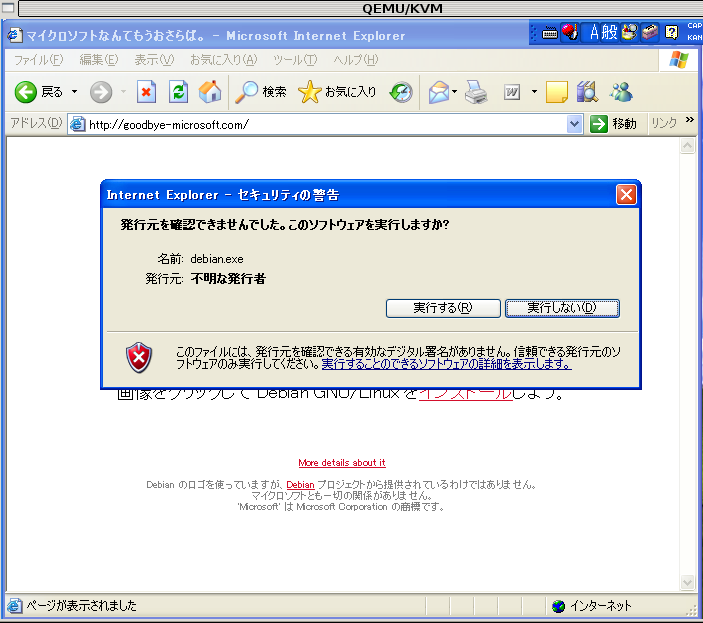
\includegraphics[width=10cm]{image200703/goodbyemicrosoftcom3.png}
\end{frame}
\begin{frame}[containsverbatim]{goodbye-microsoft.com を試す}
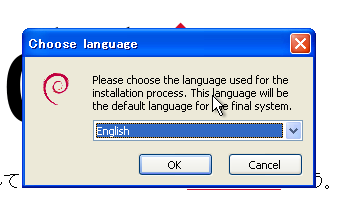
\includegraphics[width=10cm]{image200703/goodbyemicrosoftcom4.png}\\
\end{frame}
\begin{frame}[containsverbatim]{goodbye-microsoft.com を試す}
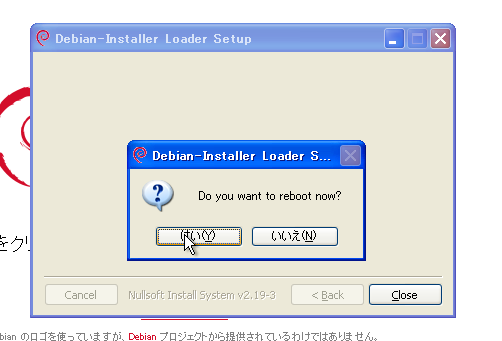
\includegraphics[width=10cm]{image200703/goodbyemicrosoftcom5.png}
\end{frame}
\begin{frame}[containsverbatim]{goodbye-microsoft.com を試す}
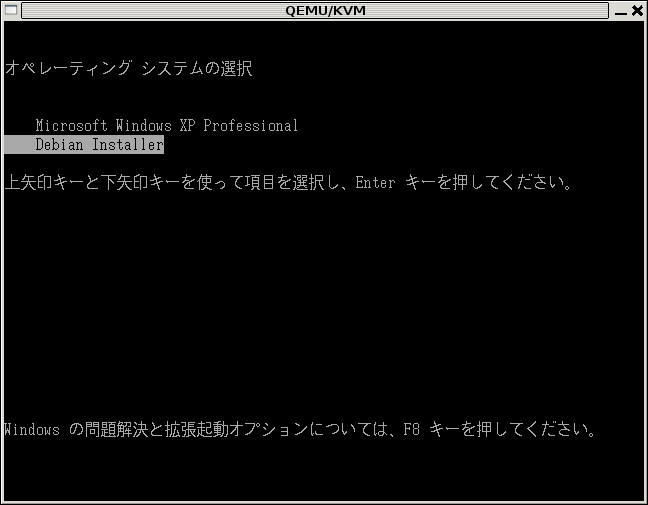
\includegraphics[width=10cm]{image200703/goodbyemicrosoftcom6.png}\\
\end{frame}
\begin{frame}[containsverbatim]{goodbye-microsoft.com を試す}
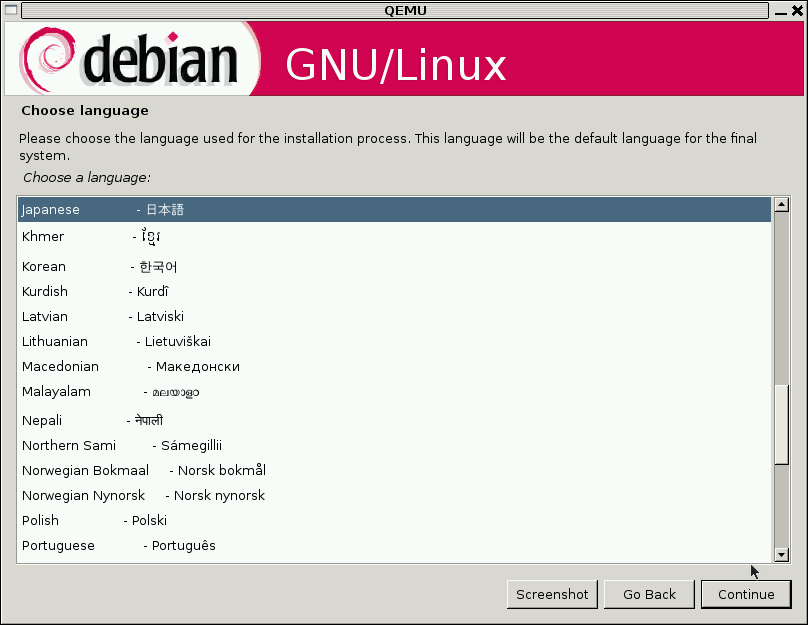
\includegraphics[width=10cm]{image200703/goodbyemicrosoftcom7.png}
\end{frame}
\begin{frame}[containsverbatim]{goodbye-microsoft.com を試す}
無事 goodbye-microsoft.com が稼働することを確認できました。
\end{frame}

\begin{frame}[containsverbatim]{PaSoRi を試す}

qemu でホストOSの USB デバイスをゲストOSのUSBデバイスとして見せることが
 でき、KVMでも同様。PaSoRiできるじゃん!

\begin{verbatim}
 qemu-img create -f qcow -b winxp.cow winxp.cow-work
 kvm -localtime \
 -hda winxp.cow -m 400 \
 -redir tcp:3389::3389 \
 -usb -usbdevice host:054c:01bb
\end{verbatim}

注1: kvm を実行する場合には /dev/kvm と /proc/bus/usb にアクセス権限が
 必要

注2: 054c:01bb は PaSoRi の USB デバイスとしてのベンダーとID番号
\end{frame}

\begin{frame}{PaSoRi を試す: PiTaPa}
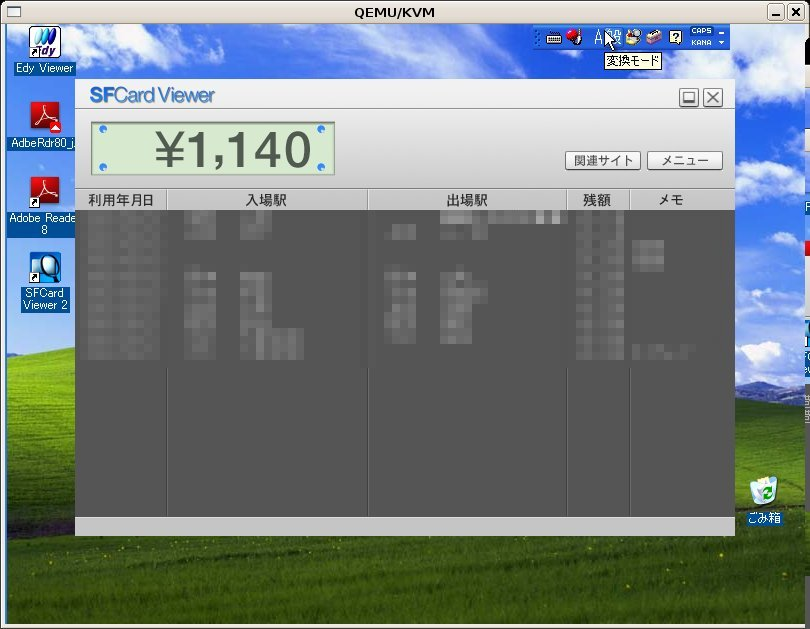
\includegraphics[width=10cm]{image200703/edy1.jpg}
\end{frame}

\begin{frame}{PaSoRi を試す: Edyチャージ}
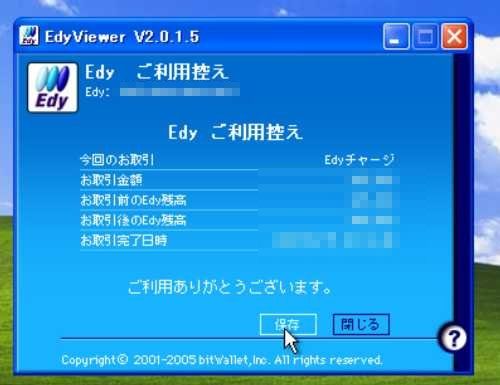
\includegraphics[width=10cm]{image200703/edy2.jpg}
\end{frame}

\begin{frame}{KVMの詳細の濃い話}

QEMU 三段活用
\begin{itemize}
 \item qemu
 \item kqemu
 \item kvm
\end{itemize}
\end{frame}

\begin{frame}{qemu}
\begin{minipage}[]{0.4\hsize}
  \includegraphics[width=0.9\hsize]{image200703/qemu.eps}
\end{minipage}
\begin{minipage}[]{0.55\hsize}
 実行対象のコード解析、コードを生成して実行

 通常のエミュレータといわれるアプリケーション

 基本的傾向として、ネイティブに対してオーバヘッドがあり、遅い

類似事例:
 aranym, bochs, 
 Java VM など
\end{minipage}
\end{frame}

\begin{frame}{kqemu}
\begin{minipage}[]{0.4\hsize}
 \includegraphics[width=0.9\hsize]{image200703/kqemu.eps}
\end{minipage}
\begin{minipage}[]{0.55\hsize}
 実行対象のコードをユーザ空間で実行してしまい、実行できない命令が発行さ
 れたら発生する exception をトラップすることで実装

 仮想モードにフルバーチャライゼーションモードと通常のモードがあり、'-
 kernel-kqemu'オプションで指定。通常のモードだとユーザ空間のみ直接実行で
 カーネル空間についてはエミュレーション。フルバーチャライゼーションモー
 ドだとゲストOSのカーネル空間もユーザ空間で直接実行するそうだ

類似事例:
 VMWare 等
\end{minipage}
\end{frame}

\begin{frame}{kvm}
\begin{minipage}[]{0.4\hsize}
 \includegraphics[width=0.9\hsize]{image200703/kvm.eps}
\end{minipage}
\begin{minipage}[]{0.55\hsize}
 実行対象のコードを CPU の仮想化機能を活用して実行する

類似事例:
 Xen 等
\end{minipage}
\end{frame}

\begin{frame}{濃い話2}
 平さん:KVMソースネタ
\end{frame}

\begin{frame}{最後に}
 \begin{itemize}
  \item ブースを出しています。
	詳しく濃い話がしたいかたはブースにて。
  \item 勉強会を開催しています。\\
	Debian 勉強会の月例会、次回は
	2007年4月21日(土曜日) 18:00-21:00 予定です。
  \item	仮想化友の会の次回は
	未定?
 \end{itemize}
\end{frame}

\end{document}
